\documentclass[man, fleqn, noextraspace,floatsintext]{apa6}
\usepackage{lmodern}
\usepackage{amssymb,amsmath}
\usepackage{ifxetex,ifluatex}
\usepackage{fixltx2e} % provides \textsubscript
\ifnum 0\ifxetex 1\fi\ifluatex 1\fi=0 % if pdftex
  \usepackage[T1]{fontenc}
  \usepackage[utf8]{inputenc}
\else % if luatex or xelatex
  \ifxetex
    \usepackage{mathspec}
  \else
    \usepackage{fontspec}
  \fi
  \defaultfontfeatures{Ligatures=TeX,Scale=MatchLowercase}
\fi
% use upquote if available, for straight quotes in verbatim environments
\IfFileExists{upquote.sty}{\usepackage{upquote}}{}
% use microtype if available
\IfFileExists{microtype.sty}{%
\usepackage{microtype}
\UseMicrotypeSet[protrusion]{basicmath} % disable protrusion for tt fonts
}{}
\usepackage{hyperref}
\hypersetup{unicode=true,
            pdftitle={What explains happiness? The relationships between happiness and marrige, health, trust, and family savings},
            pdfauthor={Asha Yadav, Joanna, \& Thuy},
            pdfkeywords={happiness},
            pdfborder={0 0 0},
            breaklinks=true}
\urlstyle{same}  % don't use monospace font for urls
\usepackage{graphicx,grffile}
\makeatletter
\def\maxwidth{\ifdim\Gin@nat@width>\linewidth\linewidth\else\Gin@nat@width\fi}
\def\maxheight{\ifdim\Gin@nat@height>\textheight\textheight\else\Gin@nat@height\fi}
\makeatother
% Scale images if necessary, so that they will not overflow the page
% margins by default, and it is still possible to overwrite the defaults
% using explicit options in \includegraphics[width, height, ...]{}
\setkeys{Gin}{width=\maxwidth,height=\maxheight,keepaspectratio}
\IfFileExists{parskip.sty}{%
\usepackage{parskip}
}{% else
\setlength{\parindent}{0pt}
\setlength{\parskip}{6pt plus 2pt minus 1pt}
}
\setlength{\emergencystretch}{3em}  % prevent overfull lines
\providecommand{\tightlist}{%
  \setlength{\itemsep}{0pt}\setlength{\parskip}{0pt}}
\setcounter{secnumdepth}{0}
% Redefines (sub)paragraphs to behave more like sections
\ifx\paragraph\undefined\else
\let\oldparagraph\paragraph
\renewcommand{\paragraph}[1]{\oldparagraph{#1}\mbox{}}
\fi
\ifx\subparagraph\undefined\else
\let\oldsubparagraph\subparagraph
\renewcommand{\subparagraph}[1]{\oldsubparagraph{#1}\mbox{}}
\fi

%%% Use protect on footnotes to avoid problems with footnotes in titles
\let\rmarkdownfootnote\footnote%
\def\footnote{\protect\rmarkdownfootnote}


  \title{What explains happiness? The relationships between happiness and
marrige, health, trust, and family savings}
    \author{Asha Yadav\textsuperscript{1}, Joanna\textsuperscript{1}, \&
Thuy\textsuperscript{1}}
    \date{}
  
\shorttitle{What explains happiness?}
\affiliation{
\vspace{0.5cm}
\textsuperscript{1} University of Oregon}
\keywords{happiness\newline\indent Word count: X}
\usepackage{csquotes}
\usepackage{upgreek}
\captionsetup{font=singlespacing,justification=justified}

\usepackage{longtable}
\usepackage{lscape}
\usepackage{multirow}
\usepackage{tabularx}
\usepackage[flushleft]{threeparttable}
\usepackage{threeparttablex}

\newenvironment{lltable}{\begin{landscape}\begin{center}\begin{ThreePartTable}}{\end{ThreePartTable}\end{center}\end{landscape}}

\makeatletter
\newcommand\LastLTentrywidth{1em}
\newlength\longtablewidth
\setlength{\longtablewidth}{1in}
\newcommand{\getlongtablewidth}{\begingroup \ifcsname LT@\roman{LT@tables}\endcsname \global\longtablewidth=0pt \renewcommand{\LT@entry}[2]{\global\advance\longtablewidth by ##2\relax\gdef\LastLTentrywidth{##2}}\@nameuse{LT@\roman{LT@tables}} \fi \endgroup}


\usepackage{lineno}

\linenumbers
\raggedbottom
\setlength{\parskip}{0pt}

\authornote{We thank Dr.~Nese for his guidance in this
project. All mistakes remain ours.

Correspondence concerning this article should be addressed to Asha
Yadav, Postal address. E-mail:
\href{mailto:ayadav@uoregon.edu}{\nolinkurl{ayadav@uoregon.edu}}}

\abstract{
abstract goes here


}

\begin{document}
\maketitle

\section{Introduction}\label{introduction}

Study of happiness and its causal factors has been flourished in recent
years. Scholars have studied the relationship between happines and
variables ranging from the political system to cultural and economic
factors to (Inglehart, 2009; Schyns, 1998).This project explores the
relationship between happiness and some candidate variables, namely
marital status, level of family savings, status of heath, and level of
trust.

\section{Methods}\label{methods}

This project drew from survey data from the
\href{http://www.worldvaluessurvey.org/WVSContents.jsp}{World Values
Survey}. This is a survey of more than 85,000 respondents across 60
countries and societies around the world. We used data from the most
recent wave which can be accessed
\href{http://www.worldvaluessurvey.org/WVSDocumentationWV6.jsp}{here}.
Our data analyses are descriptive and exploratory.\\
\#\# Data analysis and results

\subsubsection{Happiness and trust}\label{happiness-and-trust}

In this section we examine the relationship between happiness and trust.
Johnson (2012) finds that \enquote{trust as measured by the World Values
Survey is positively correlated with experimentally measured trust}.

Out of the total 76222 people, only slightly more than 24.47 percent say
they can trust most of the people around them, while 75.53 are caucious
about the society. Interstingly, there are more people feel happy in
life in the latter group than those in the former. Figure 1, below,
indicates such difference.

\begin{figure}
\centering
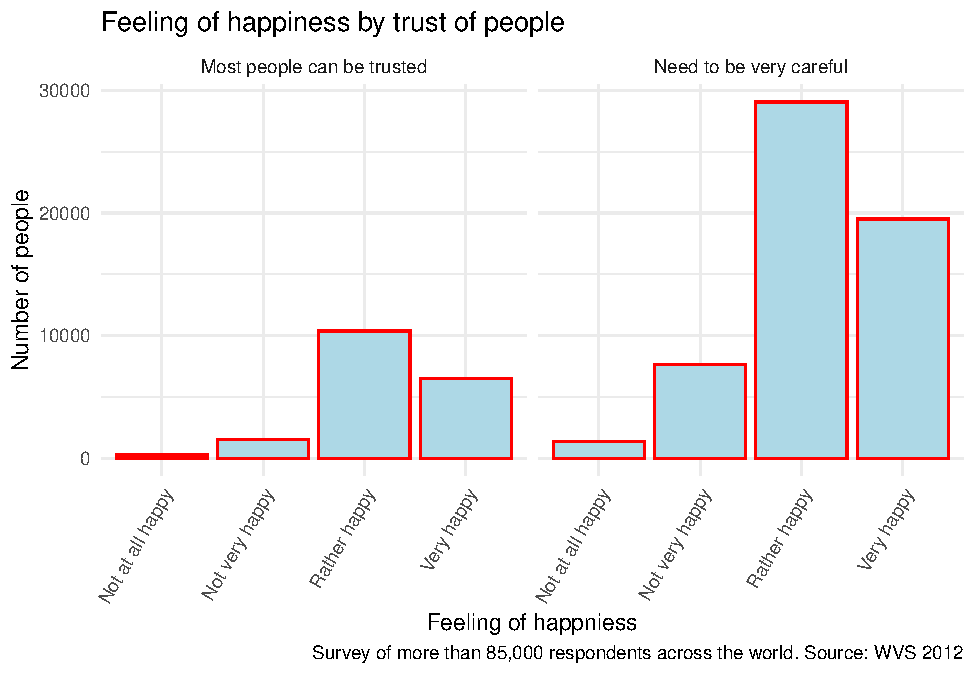
\includegraphics{610_final_files/figure-latex/unnamed-chunk-1-1.pdf}
\caption{}
\end{figure}

\subsubsection{Happiness and health
status}\label{happiness-and-health-status}

Our data suggest a positive correlation between health status and
perceived level of happiness. Figure 2, below, clearly indicates that
most of people who rated their health status as \enquote{good} also felt
happy.
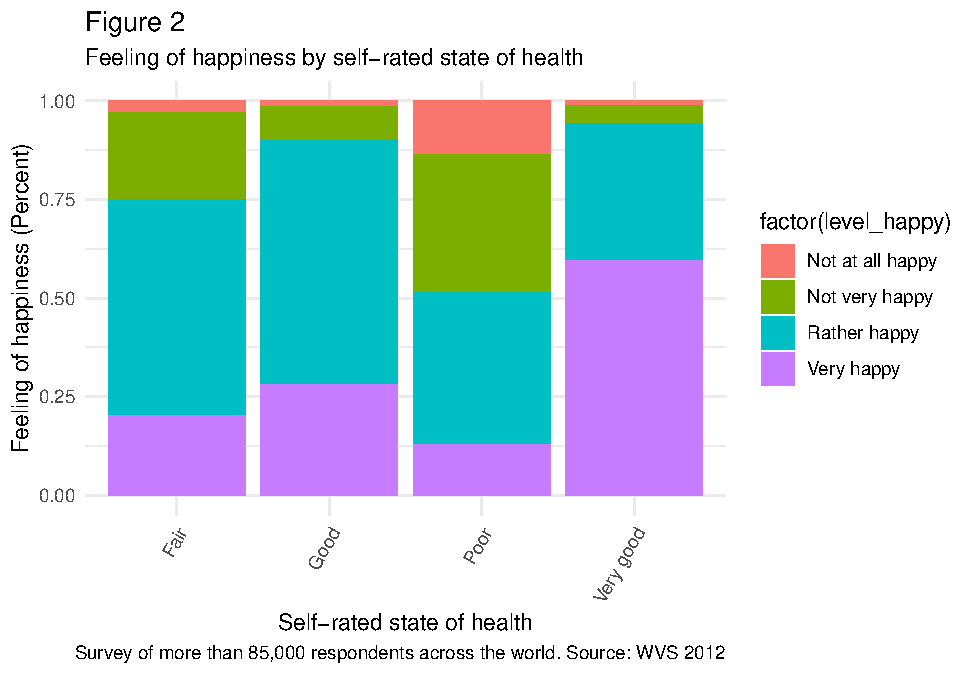
\includegraphics{610_final_files/figure-latex/unnamed-chunk-2-1.pdf}

\subsubsection{Happiness and family
savings}\label{happiness-and-family-savings}

Of the 76222 survey participants, the majority (45.48) reported just
getting by financially, while 28.72 saved money. The remainder spent
either some (14.87) or all (10.93) of their savings.

Table 1 shows happiness levels by level of family savings. Relationships
between happiness levels and family savings are explored in Figure 3.
Here, we see that of those reporting the lowest levels of happiness (Not
at all happy, Not very happy), most had spent all of their family
savings. On the other hand, of those reporting the highest level of
happiness (Very happy), the highest percentage were those in the
strongest financial position - those who saved money.

\begin{table}[tbp]
\begin{center}
\begin{threeparttable}
\caption{\label{tab:happiness by family APA table}}
\begin{tabular}{lllll}
\toprule
family\_savings & \multicolumn{1}{c}{feeling\_of\_happiness} & \multicolumn{1}{c}{n} & \multicolumn{1}{c}{total} & \multicolumn{1}{c}{percent}\\
\midrule
Just get by & Not at all happy & 813 & 34669 & 2.35\\
Just get by & Not very happy & 4650 & 34669 & 13.41\\
Just get by & Rather happy & 18661 & 34669 & 53.83\\
Just get by & Very happy & 10545 & 34669 & 30.42\\
Save money & Not at all happy & 203 & 21889 & 0.93\\
Save money & Not very happy & 1449 & 21889 & 6.62\\
Save money & Rather happy & 11060 & 21889 & 50.53\\
Save money & Very happy & 9177 & 21889 & 41.93\\
Spent savings and borrowed money & Not at all happy & 400 & 8333 & 4.80\\
Spent savings and borrowed money & Not very happy & 1577 & 8333 & 18.92\\
Spent savings and borrowed money & Rather happy & 3867 & 8333 & 46.41\\
Spent savings and borrowed money & Very happy & 2489 & 8333 & 29.87\\
Spent some savings and borrowed money & Not at all happy & 207 & 11331 & 1.83\\
Spent some savings and borrowed money & Not very happy & 1471 & 11331 & 12.98\\
Spent some savings and borrowed money & Rather happy & 5853 & 11331 & 51.65\\
Spent some savings and borrowed money & Very happy & 3800 & 11331 & 33.54\\
\bottomrule
\end{tabular}
\end{threeparttable}
\end{center}
\end{table}

\begin{figure}
\centering
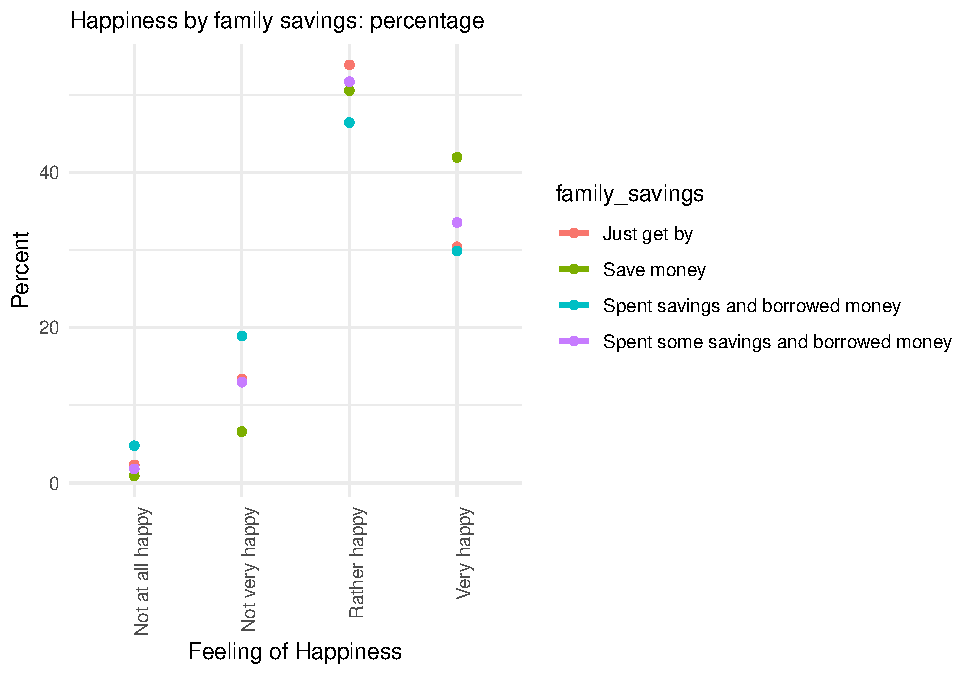
\includegraphics{610_final_files/figure-latex/happiness by family savings tables and figures-1.pdf}
\caption{}
\end{figure}

\section{Discussion}\label{discussion}

Our results illuminate a number of connections between happiness levels
and other life factors such as trust of others, family financial status,
and health.

Data for happiness levels overall were normally distributed, with the
majority of participants reporting a moderate level of happiness, and
fewer reporting very low or very high levels of happiness. This pattern
continued to be evident when data were grouped by our independent
variables.

Contrary to the conventional belief that people who feel they can trust
people around them should feel more secured, hence happier. The data
shows us somewhat the opposite. Those who say they should be careful
with the fellows surrounding them indicates higher level of happiness.

Results indicate that good health is associated with greater feelings of
happiness. This affirms prior research by Gandelman and
Hernández-Murillo (2013) which found a strong relationship between
self-rated health status and perceived life quality.

Results also suggest a positive relationship between family financial
circumstances and happiness. Prior research has demonstrated a positive
association between income and well-being, although the mechanisms for
this remain unclear (Diener, 2010). Our results build on this work by
indicating that degree to which families are able to save money, or the
degree to which they must deplete savings and/or take out loans, are
areas worthy of further study.

Our results should be interpreted with caution. Because we are beginners
in using R, data analyses are, so far, only descriptive. Linear models
are needed to explore whether the relationships suggested here are
statistically significant. Furthermore, even if they were, these data
are cross-sectional, so findings cannot be interpreted as indicating
causality.

\newpage

\section{References}\label{references}

\begingroup
\setlength{\parindent}{-0.5in} \setlength{\leftskip}{0.5in}

\hypertarget{refs}{}
\hypertarget{ref-diener2010}{}
Diener, N., E. (2010). Wealth and happiness across the world: Material
prosperity predicts life evaluation, whereas psychosocial prosperity
predicts positive feeling. \emph{Journal of Personality and Social
Psychology}, \emph{99}(1), 52--61.

\hypertarget{ref-gandelman2013happiness}{}
Gandelman, N., \& Hernández-Murillo, R. (2013). What do happiness and
health satisfaction data tell us about relative risk aversion?
\emph{Journal of Economic Psychology}, \emph{39}, 301--312.

\hypertarget{ref-inglehart200911}{}
Inglehart, R. (2009). 11. democracy and happiness: What causes what?
\emph{Happiness, Economics and Politics: Towards a Multi-Disciplinary
Approach}, 256.

\hypertarget{ref-johnson2012much}{}
Johnson, N. D., \& Mislin, A. (2012). How much should we trust the world
values survey trust question? \emph{Economics Letters}, \emph{116}(2),
210--212.

\hypertarget{ref-schyns1998crossnational}{}
Schyns, P. (1998). Crossnational differences in happiness: Economic and
cultural factors explored. \emph{Social Indicators Research},
\emph{43}(1-2), 3--26.

\endgroup


\end{document}
